\chapter{Từ trường, tính chất của đường sức từ}
\section{Lý thuyết trọng tâm}
\subsection{Nam châm}
\begin{center}
	
\includegraphics[scale=0.8]{../figs/VN11-PH-24-L-016-1-h103.jpg}
\end{center}

 Nam châm thường là các chất (hoặc là các hợp chất của chúng) như sắt, niken, côban, mangan,...

 Mỗi nam châm bao giờ cũng có hai cực phân  biệt. Hai cực của nam châm được đặt tên là cực Bắc, kí hiệu là chữ N và cực nam, kí hiệu là chữ S.

 Hai cực của nam châm đặt gần nhau sẽ đẩy nhau khi chúng cùng tên và hút nhau khi chúng khác tên. Lực tương tác đó được gọi là lực từ và các nam châm được gọi là có từ tính.

\subsection{Từ tính của dây dẫn có dòng điện}

 Giữa hai dây dẫn có dòng điện, giữa hai nam châm, giữa một dòng điện và một nam châm đều có lực tương tác; những lực tương tác ấy gọi là lực từ, dòng điện và nam châm đều có từ tính.


\subsection{Từ trường}

Từ trường là một dạng vật chất tồn tại trong không gian mà biểu hiện cụ thể là sự xuất hiện của lực từ tác dụng lên dòng điện hay một nam châm đặt trong nó. 

Người ta quy ước: hướng của từ trường tại một điểm là hướng Nam - Bắc của kim nam châm nhỏ nằm cân bằng tại điểm đó.

\subsection{Đường sức từ}
\subsubsection{Định nghĩa}

\begin{center}
	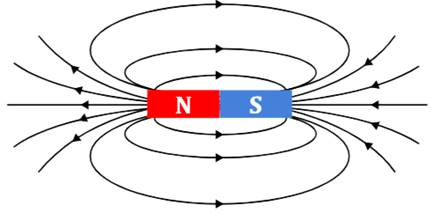
\includegraphics[scale=0.8]{../figs/VN11-PH-24-L-016-1-h104.jpg}
\end{center}
Đường sức từ là những đường vẽ ở trong không gian có từ trường sao cho tiếp tuyến tại mỗi điểm có phương trùng với phương của từ trường tại điểm đó.  
\subsubsection{Các tính chất của đường sức}
Các đường sức có những tính chất sau:

	\begin{itemize}
	\item Tại mỗi điểm trong không gian có từ trường chỉ vẽ được một và chỉ một đường sức từ.
	\item Các đường sức từ là những đường cong khép kín hoặc vô hạn ở hai đầu.
	\item Chiều của các đường sức từ tuân theo những quy tắc xác định (quy tắc nắm tay phải, quy tắc vào Nam ra Bắc).
	\item 	Quy ước vẽ các đường sức từ sao cho chỗ nào từ trường mạnh thì các đường sức từ mau và chỗ nào từ trường yếu thì các đường sức từ thưa.
\end{itemize}

\section{Bài tập}
\begin{dang}{Từ trường, tính chất của đường sức từ}
\end{dang}

\textbf{Phương pháp giải}

Ghi nhớ tính chất và các cực của nam châm.

Ghi nhớ từ tính của nam châm và dòng điện.

Ghi nhớ khái niệm từ trường và hướng của từ trường.

Ghi nhớ đường sức từ và tính chất của đường sức từ.

\vspace*{1em}
\viduii{1}
{Lực nào sau đây không phải lực từ?
\begin{mcq}(1)
	\item Lực Trái đất tác dụng lên kim nam châm ở trạng thái tự do làm nó định hướng theo phương bắc nam. 
	\item Lực hai dây dẫn mang dòng điện tác dụng lên nhau.
	\item Lực nam châm tác dụng lên dây dẫn bằng nhôm mang dòng điện.
	\item Lực Trái Đất tác dụng lên vật nặng.
\end{mcq}}
{\begin{center}
		\textbf{Hướng dẫn giải:}
\end{center}

Lực Trái Đất tác dụng lên vật nặng là trọng lực chứ không phải lực từ.	

\textbf{	Đáp án: D.}
}

\viduii{1}
{	
Từ trường là dạng vật chất tồn tại trong không gian và
	\begin{mcq}
		\item  tác dụng lực hút lên các vật.
		\item tác dụng lực điện lên điện tích.
		\item tác dụng lực từ lên nam châm và dòng điện.
		\item tác dụng lực đẩy lên các vật đặt trong nó.
	\end{mcq}
}{	
\begin{center}
		\textbf{Hướng dẫn giải:}
\end{center}
	
Từ trường là dạng vật chất tồn tại trong không gian và tác dụng lực từ lên nam châm và dòng điện.
	
\textbf{Đáp án: C.}
	
}

\viduii{1}
	{
	Các đường sức từ là các đường vẽ trong không gian có từ trường sao cho
	\begin{mcq}
		\item pháp tuyến tại mọi điểm trùng với hướng của từ trường tại điểm đó.
		\item tiếp tuyến tại mọi điểm trùng với hướng của từ trường tại điểm đó.
		\item pháp tuyến tại mỗi điểm tạo với hướng của từ trường một góc không đổi.
		\item tiếp tuyến tại mọi điểm tạo với hướng của từ trường một góc không đổi.
	\end{mcq}
}
{\begin{center}
		\textbf{Hướng dẫn giải:}
\end{center}
	
	Các đường sức từ là các đường vẽ trong không gian có từ trường sao cho tiếp tuyến tại mọi điểm trùng với hướng của từ trường tại điểm đó.
	
\textbf{	Đáp án: B.}
	
}

\viduii{1}
	{
	Đường sức từ không có tính chất nào sau đây?
	\begin{mcq}
		\item Qua mỗi điểm trong không gian chỉ vẽ được một đường sức.
		\item Các đường sức là các đường cong khép kín hoặc vô hạn ở hai đầu.
		\item Chiều của các đường sức là chiều của từ trường. 
		\item Các đường sức của cùng một từ trường có thể cắt nhau.
	\end{mcq}
}{
\begin{center}
		\textbf{Hướng dẫn giải:}
\end{center}

	Các đường sức của cùng một từ trường không cắt nhau.
	
\textbf{	Đáp án: D.}
	
}




